\section{Setup Environment}

We simulate all path finding processes based on the framework of 
GridWorld\cite{web:gridworld}, an AP case study project from collegeboard
\footnote{https://www.collegeboard.org/}. It provides graphical user interface 
based on Java AWT where visual objects can interact and perform customized 
actions in a two-dimensional grid map. In the next part, we will first illustrate
original GridWorld framework and our enhancement of displaying colored path.
This mainly involves the engineering work, so if you want to directly delve 
into algorithm analysis, please skip it.

\subsection{GridWorld Architecture and Modification}

The framework structure of original GridWorld project are divided into four parts: 
Actor, Grid, GUI and World, as shown in Figure \ref{fig:framework-structure}.
The Actor package contains objects whose behavior on the map can be arbitrarily 
defined by rewriting following method in each inherited class:

\begin{lstlisting}
%%@Override%%
public void act()
\end{lstlisting}

\begin{figure}[ht]
\centering
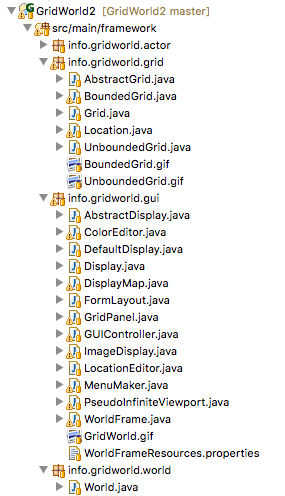
\includegraphics[width=0.5\textwidth]{framework-structure}
\caption{GridWorld package structure}
\label{fig:framework-structure}
\end{figure}

The Grid package defines bounded grid
map features and connection to actors. The GUI package encapsulates low-level
Java AWT to provide APIs for visualization and interactions of map and actors.
The World package provides high-level integration of actors and world.

In order to visualize the presumed unblocked path and the set of nodes expanded
and explored after each planning, we enhance the $GridPanel$ class in the 
GUI package by implementing following method:

\begin{lstlisting}
private void drawColoredLocations(Graphics2D g2)
\end{lstlisting}

Meanwhile, following five abstract methods are added to $Grid$ class so that
inherited classes like $BoundedGrid$ and $UnboundedGrid$ should provide 
implementation of how to configure colors on each grid.
\begin{lstlisting}
ArrayList<Location> getColoredLocations();
Color getColor(Location loc);
void putColor(Location loc, Color color);
void removeColor(Location loc);
void resetColors();
\end{lstlisting}


\subsection{Maze Generation Algorithm}

\subsection{How to Run}

Our project is 
